%%%%%%%%%%%%%%%%%%%%%%%%%%%%%%%%%%%%%%%%%%%%%%%%%%%%%%%%%%%%%%%%%%%%%%%%%%%%%%%%
%2345678901234567890123456789012345678901234567890123456789012345678901234567890
%        1         2         3         4         5         6         7         8

\documentclass[letterpaper, 10 pt, conference]{ieeeconf}  % Comment this line out if you need a4paper

%\documentclass[a4paper, 10pt, conference]{ieeeconf}      % Use this line for a4 paper

\IEEEoverridecommandlockouts                              % This command is only needed if 
                                                          % you want to use the \thanks command

\overrideIEEEmargins                                      % Needed to meet printer requirements.

% See the \addtolength command later in the file to balance the column lengths
% on the last page of the document

% The following packages can be found on http:\\www.ctan.org
%\usepackage{graphics} % for pdf, bitmapped graphics files
%\usepackage{epsfig} % for postscript graphics files
%\usepackage{mathptmx} % assumes new font selection scheme installed
%\usepackage{times} % assumes new font selection scheme installed
%\usepackage{amsmath} % assumes amsmath package installed
%\usepackage{amssymb}  % assumes amsmath package installed
\usepackage{graphicx}
\usepackage[export]{adjustbox}
\graphicspath{ {images/} }


\title{\LARGE \bf
Marine Multi-robot Patrolling
}

\author{Pin-Wei Chen$^{1}$, Ni-Ching Lin$^{2}$ and Bo-Sheng She$^{3}$ % <-this % stops a space
\thanks{*This work was supported by the Robotics Master Program in National Chiao Tung University, Taiwan}% <-this % stops a space
\thanks{$^{1}$Pin-Wei Chen, National Chiao Tung University, Taiwan.		{\tt\small ccpwearth@gmail.com}}%
}


\begin{document}



\maketitle
\thispagestyle{empty}
\pagestyle{empty}


\section{INTRODUCTION \& MOTIVATION}

Multi-robot patrolling is an potential idea, I can apply this project to surveillance, security, production line, etc. I realize that robot can help us with something routine and cycling, such as patrolling, which I should patroll lots of nodes again and again. As a result, I come up with this idea, trying to build a multi-robot patrolling system in ROS, and also combine this system with duckietown.

\section{SYSTEM ARCHITECTURE \& EQUIPMENTS}

\subsection{SYSTEM ARCHITECTURE}


This section explains the approaches in both "hardware" or "software systems". You should explain here the key components/modules and they are working together (typically in a flowchart or a system diagram). Wherever possible, the methods and tasks to be performed should be outlined in logical sequence and explained in detail. Do not assume the reviewer will fill in the gaps in your logic. A ROS system diagram generated by rqt\_graph~\cite{rqt-graph} may be useful (you can learn "rqt" easily from google).

\subsection{EQUIPMENTS} 

The robot I use is Moified from duckiebot, I replace the dagu motor with JGB37-520 motor which have an encoder in it Fig.~\ref{figure:JGB37-520}. In addition, I use yellow lines and black background as our patrol map, and I use apriltags as the patroll nodes Fig.~\ref{figure:map}. In software part, I use ROS kinetic and ubuntu 16.04 LTS as my develop enviromnet.

\begin{figure}[h] % h means put this image here
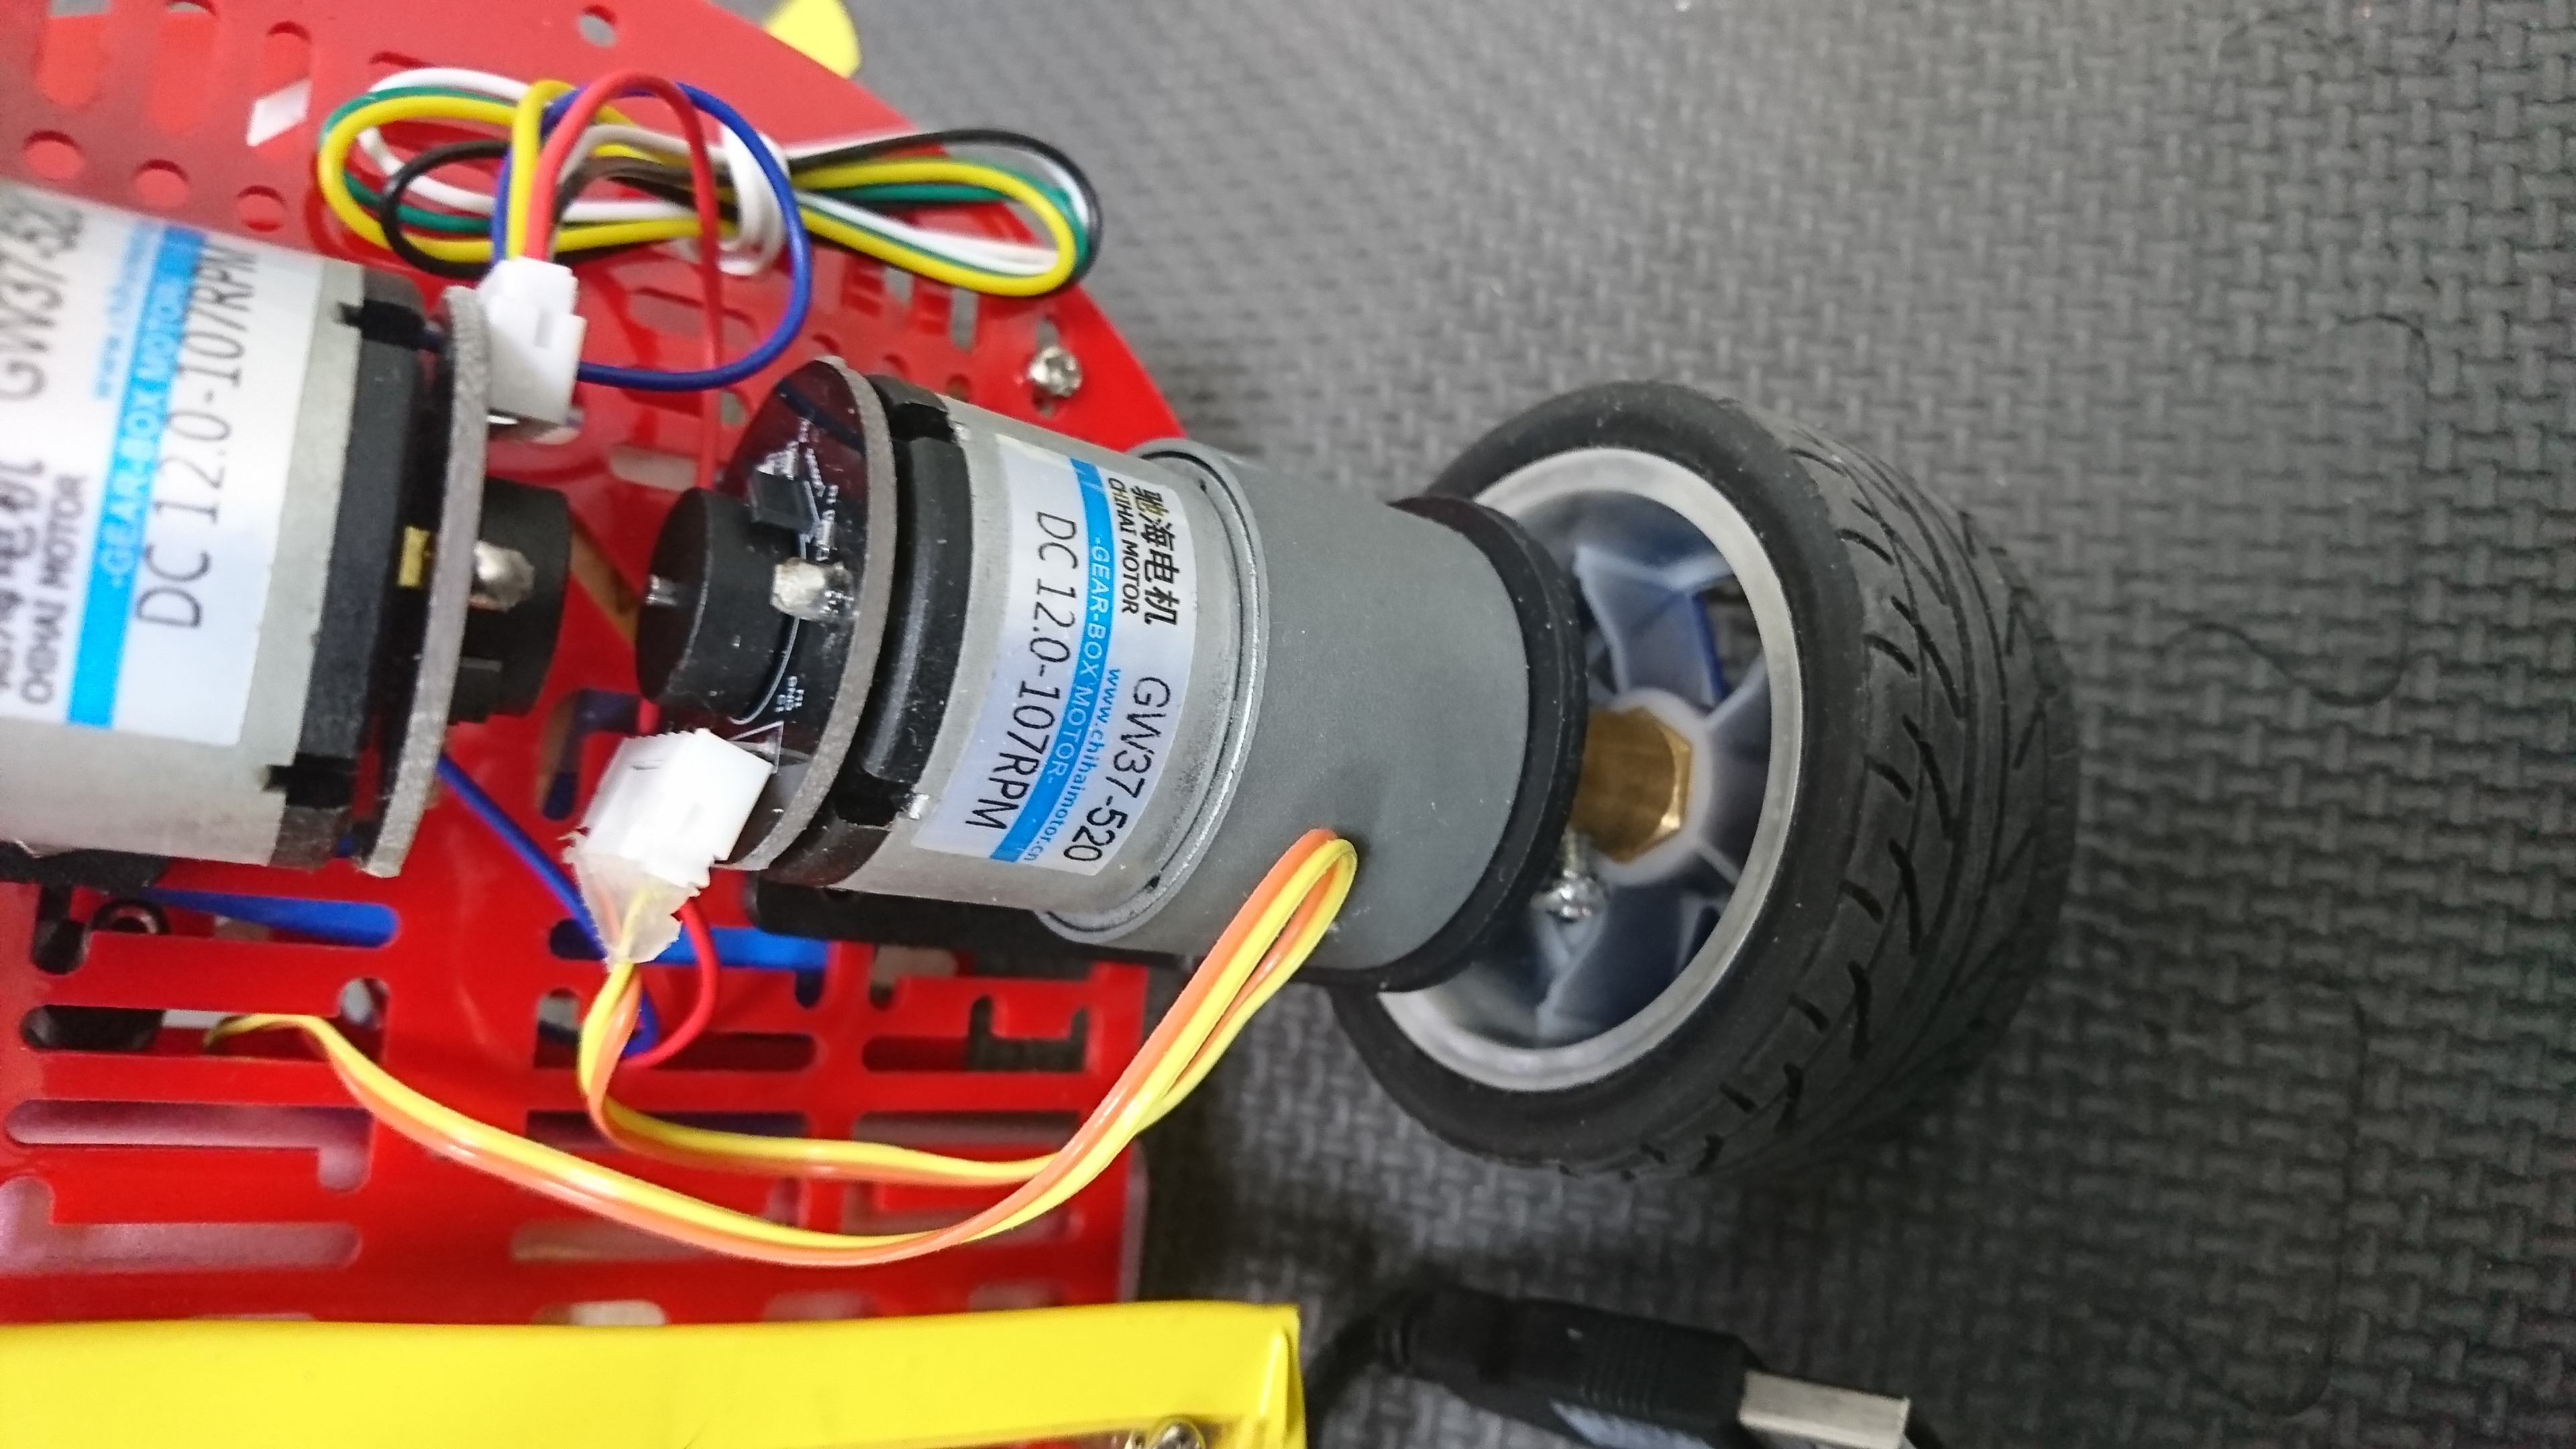
\includegraphics[width=0.8\columnwidth]{JGB37-520}
\centering
\caption{JGB37-520 encoder motor}
 \label{figure:JGB37-520}
\end{figure}

\begin{figure}[t] % t means put this image at the top 
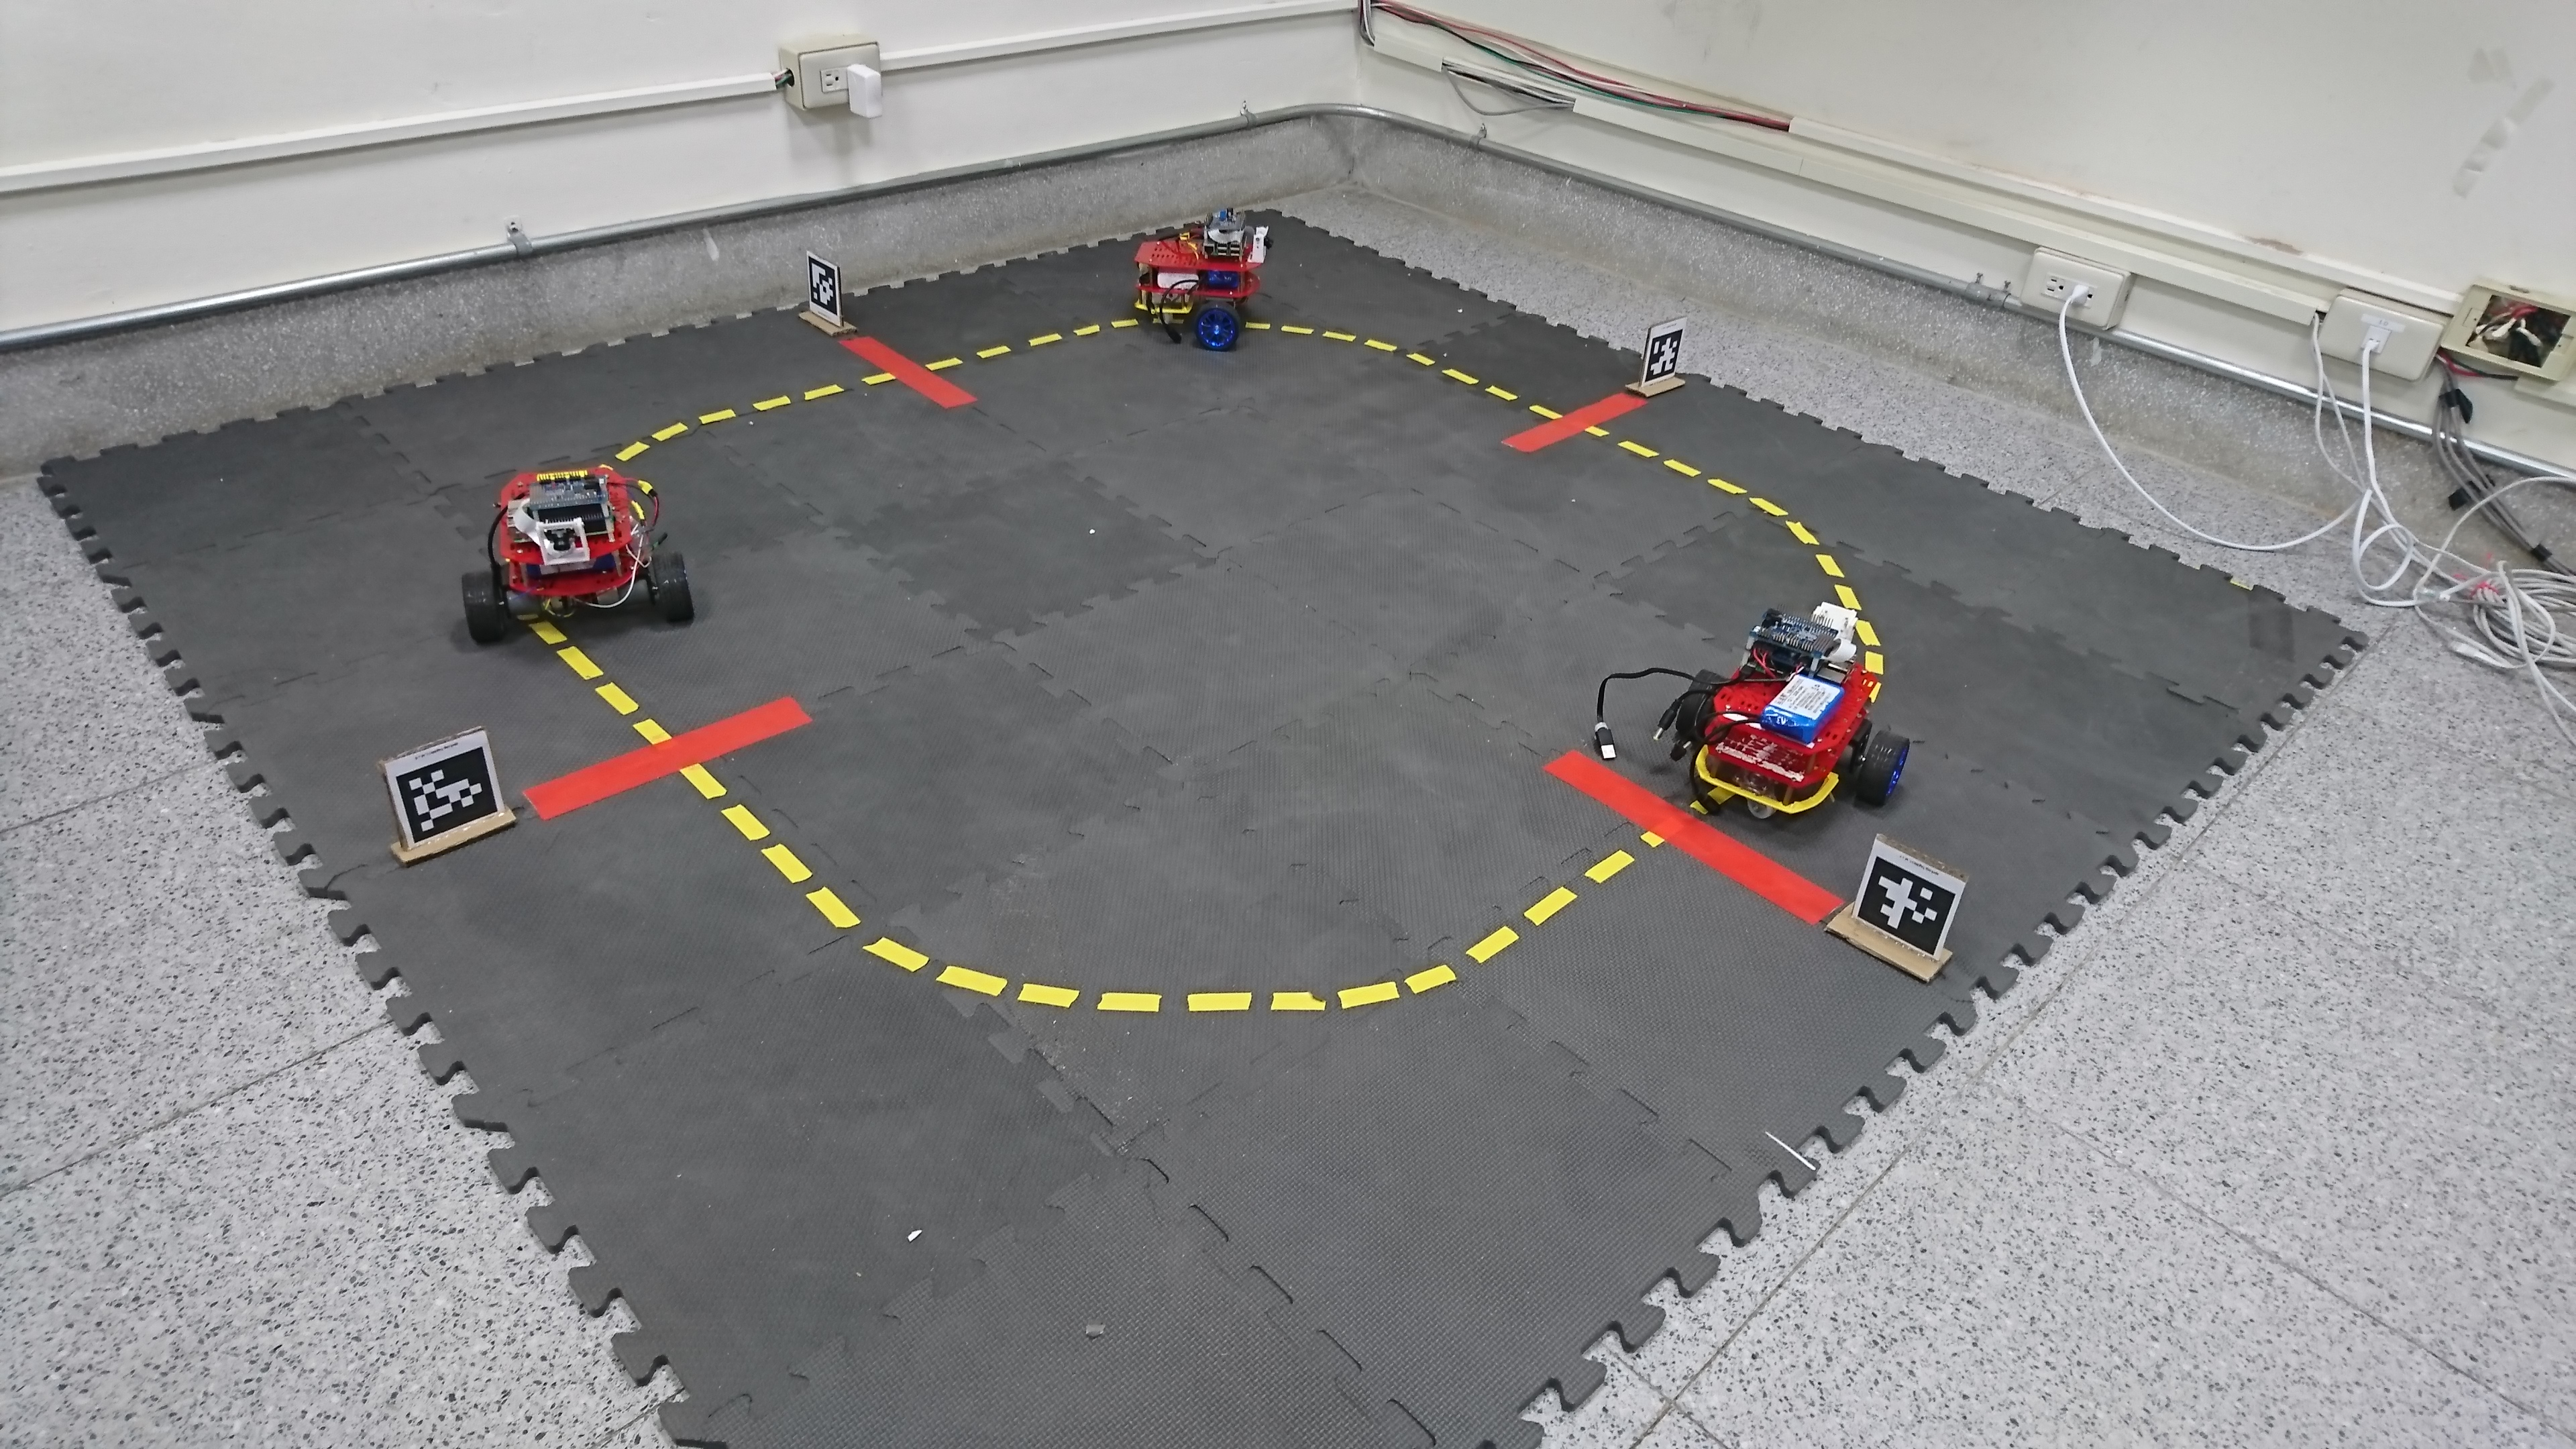
\includegraphics[width=0.8\columnwidth]{map}
\centering
\caption{Teaser figure: this figure is the most important one in the paper. It gives your readers the first impression of this work. The teaser generally includes the overview of the proposed approach and the key contributions. It appears at the upper right of the first page.}
\label{figure:map}
\end{figure}

\section{SPECIFIC AIMS}

\begin{itemize}
\item Real world patrolling system
\end{itemize}
I am trying to let multi-robot follow the yellow line and patrol multi-node(apriltags), so that each node will be patolled in approximately the same idle time. Moreover, those robot will not patol on the same lane at the same time, or they will crash with each other. 

\begin{itemize}
\item Virtual world patrolling system
\end{itemize}
I will build a virtual world and models in Gazebo, and try to move all of my patrolling system to Gazebo, so that we can easily show the concept of patrolling robot in virtual world. Moreover, we can connect real world and gazebo, so that it will easily enable us to show the status of each robot and node in gazebo.

\section{APPROACH}

(individual part)

This section should include the methods that you will need in order to reach the specific aims. You could include how you will implement your software/hardware, the design of the algorithms. Some preliminary results will be helpful as well. 

You may also state what experiments you will carry out to convince the readers that you reach the specific aims.

\section{SCHEDULE AND TEAM COLLABORATION}

(individual part)

In this section you should write a estimated timeline of your project. This schedule will be very crucial to keep up progress for your project. If you are in a team, you're encouraged to add other team members' on the timeline. It will better show the coordination of your team.
   

\addtolength{\textheight}{-12cm}   % This command serves to balance the column lengths
                                  % on the last page of the document manually. It shortens
                                  % the textheight of the last page by a suitable amount.
                                  % This command does not take effect until the next page
                                  % so it should come on the page before the last. Make
                                  % sure that you do not shorten the textheight too much.

\bibliographystyle{IEEEtran}
\bibliography{egbib}

\end{document}
